\documentclass[12pt]{article}
\usepackage[italian]{babel}
\usepackage{graphicx}
\usepackage{geometry} %To modify margins
\usepackage{multicol}
\usepackage{hyperref} %To setup table of content links
\usepackage{musixtex} %To make musical symbols

\geometry{
 a4paper,
 total={170mm,257mm},
 left=20mm,
 top=20mm,
 }

\hypersetup{
    colorlinks,
    citecolor=black,
    filecolor=black,
    linkcolor=black,
    urlcolor=black
}

\title{}
\author{Giuseppe Brusco}
\begin{document}

\begin{titlepage}
   \begin{center}
       \vspace{1cm}
	\large
      {\huge \textbf{MusicStats}}\\
       \vspace{1.5cm}
       \textbf{Giuseppe Brusco}\\
       \vspace{1.5cm}
	\textbf{A.A. 2021-2022}\\
	\vspace{0.35cm}
	\textbf{\today}
\vfill
\begin{figure}[h!]
	\begin{center}
	  
\includegraphics[scale=0.3]{media/univr}
	  
\includegraphics[scale=0.3]{media/musicStats}
	\end{center}
\end{figure}
	\vfill
 	\textbf{Elaborato per il corso di Linguaggio Programmazione LaTeX 2021/2022}
       \vspace{3cm}
      \begin{multicols}{2}
      \textbf{Università degli Studi di Verona Computer Science Department}
	\end{multicols}
   \end{center}
\end{titlepage}

\tableofcontents
\clearpage

\section{La numerologia di Johann Sebastian Bach}
La \textbf{gematria} è una scienza dell'ebraismo che studia le parole scritte in lingua ebraica e assegna loro valori numerici: questo sistema afferma che parole e/o frasi con valore numerico identico siano
correlate, o dimostrino una qualche relazione col numero stesso, applicato, per esempio, all'età di
una persona, a un anno del calendario ebraico o simili.
Questo metodo viene anche chiamato \textbf{simbolismo numerico} ed è spesso usato nella musica
rinascimentale e nel periodo Barocco.
Esempio: alla lettera A attribuiamo il valore numerico $1$, H vale $8$, ecc…
In questo modo non solo dei testi o parole possono essere tradotti in numeri ma anche le strutture
numeriche possono essere decifrate come testi.
Un esempio concreto è il nome \textbf{BACH} che espresso in numeri risulta $2138$.
Questo numero si può interpretare in diversi modi sommando tra di loro le varie cifre oppure
formando un prodotto.

\section{Numeri di Bach}
Uno dei più significativi è $14(1+2+3+8)$.

\begin{center}
\resizebox{\textwidth}{!}{%
\begin{tabular}{|c|c|c|}
  \hline
  $21*38$ & $3128$ \\
  \hline
  $41$ (J.S. Bach) & Aggiungendo zeri ad altri numeri troviamo $1400$ al posto di $14$ \\ 
  \hline
  $158$ (Johann Sebastian Bach) & $1580$ al posto di $158$\\ 
  \hline
  $480 = 2 * 3 * 1 * 80$ ($80$ è $8$ con l’aggiunta di uno zero) & Inoltre tutte le possibili permutazioni,capovolgimenti e inversioni dei $4$ numeri\\
  \hline
\end{tabular}
}
\end{center}


\section{Numero 14 come firma di Bach}
Il numero $14$ rappresenta la firma di Bach (come i suoi famosi $14$ Canoni), ma non era il solo a
firmarsi nelle sue opere (questo procedimento viene chiamato crittografia musicale).

\begin{center}
\begin{tabular}{|c|c|} 

  \hline
  si$\flat$, la, do, si$\natural$ (B, A, C, H)  & Johann Sebastian Bach \\
  \hline
  si$\natural$, la, re, re, sol (H, A, Y, D, N)  & Joseph Haydn \\ 
  \hline
  re, mi$\flat$, do, si$\natural$ (D, S, C, H) & Dmitrij Šostakovič \\
  \hline
  mi$\flat$, do, si$\natural$, la (S, C, H, A)  & Robert Schuman \\
  \hline

\end{tabular}
\end{center}
Queste permutazioni sembrano essere create apposta se si considera il senso delle lettere, ma in
musica inversioni e permutazioni di note non sono nulla di particolare.
Leggendo queste firme in senso musicale ricaviamo una sequenza di note e viceversa; così un
“nome” può diventare una “tema musicale”.
Spesso le strutture delle opere di Bach sono basate sul numero $14$ e, per via dell’analisi musicale,
si suddividono in $2$, $1$, $3$ o $8$ battute, note o unità.
Lo studio consiste di analisi fondate in gran parte su opere selezionate.

\section{Esempi della firma di Bach tramite il numero 14}

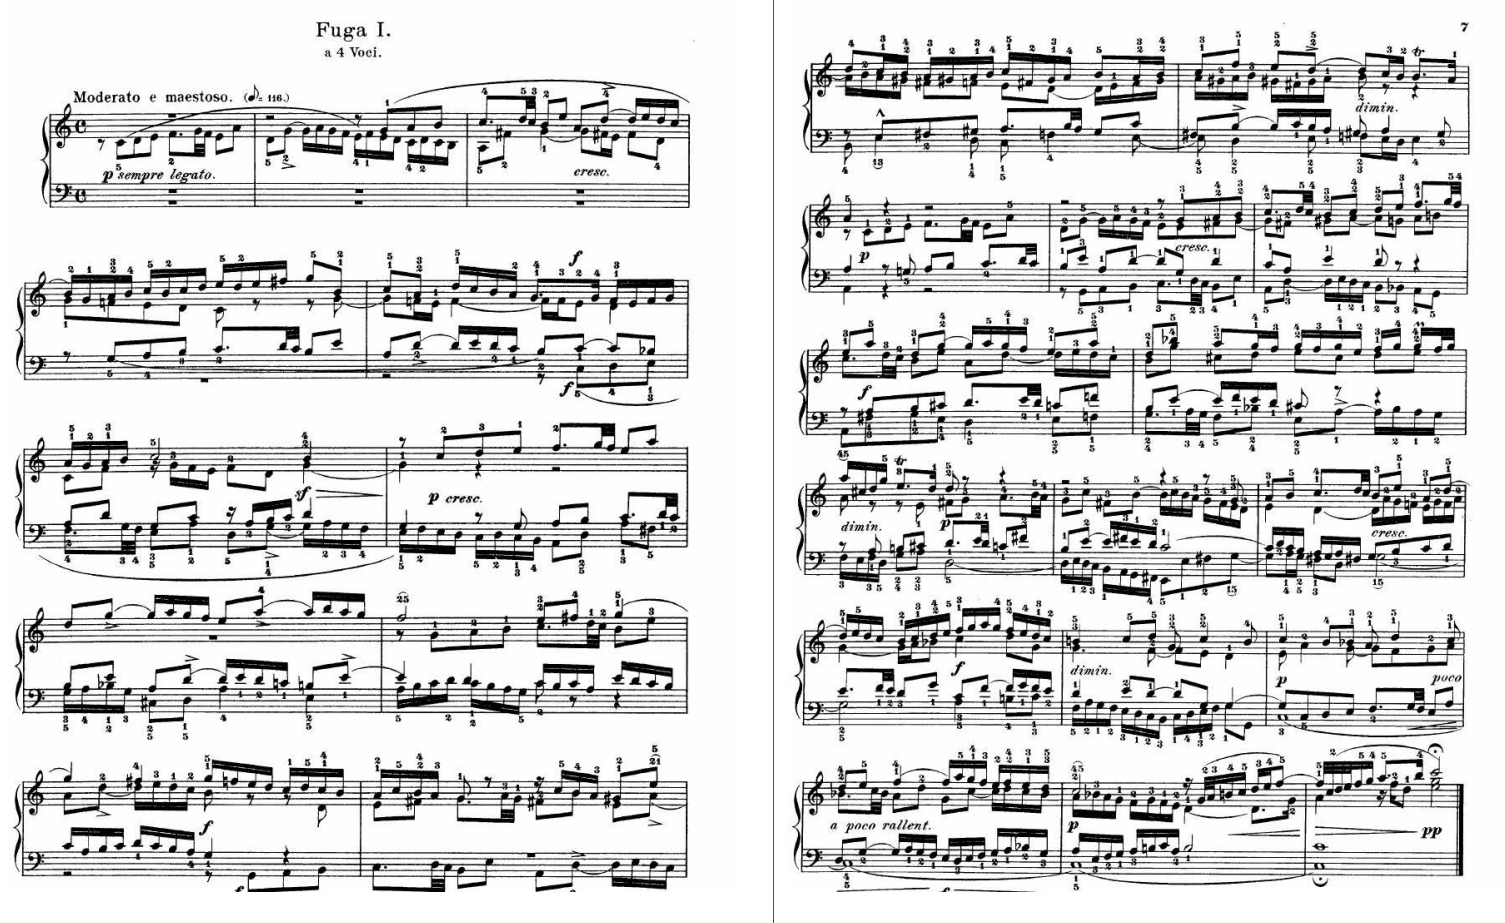
\includegraphics[scale=0.32]{media/esempio_firma.png}

Il pezzo n°1 del “Clavicembalo ben temperato” consiste in:
\begin{itemize}
    \item Preludio contenente $549$ note
    \item Fuga contenente $734$ note
\end{itemize}

Il totale ricavato è di $1283$ note: il nome di Bach ma con una sequenza diversa.
Nella fuga troviamo $24$ entrate ognuna delle quali contiene un tema di $14$ note.

\input musixtex
\setstaffs1{1} % a single stave
\setclef1{\treble} % with a treble clef
\generalmeter{\meterfrac44} % common time 4/4
\nobarnumbers % what it says
\startextract % a short music piece
% \qu = quarter note, stem up;
% \ql = quarter note, stem down;
% \Notes, \en = start and end of note line
\Notes\ds\Tqbu cde \en
\notesp\ibu0i0\qbp0f\en
\Notes\nbbbu0\qb0g\tbu0\qb0f\en
\Notes\ibu0e2\qb0e\tqu0h\en
\bar
\Notes\ibu0d2\qb0d\islurd0g\tqu0g\en
\Notes\tslur0g\ibu0h0\qb0g\en
\notes\nbbu0\qb0h\tqh0g\en
\Notes\ibbu0d{-2}\roff{\tbbu0}\qb0f\tbu0\qb0e\en
\Notes\ds\ds\qs\en
\endextract

Con una cadenza tagliente dopo l’accordo di LA minore in battuta $14$, Bach modifica la struttura in
modo tale che le entrate vengano suddivise in due gruppi rispettivamente di $10$ e $14$.
La $14$° entrata del tema alla battuta $15$ denota una particolarità: finisce dopo $7$ note invece che $14$.

\input musixtex
\setstaffs1{1}
\setclef1{\treble}
\generalmeter{\meterfrac44}
\nobarnumbers
\startextract
\Notes \qp \qp \ds \Tqbu ghi \en
\bar

\notesp\ibl0i0\qbp0j\en
\Notes\nbbbl0\qb0k\tbl0\qb0j\en
\Notes \Dqbl ij \en
\Notes \Dqbl kl \en
\notesp\ibl0k0\qbp0m\en
\Notes\nbbbl0\qb0n\tbl0\qb0m\en
\bar

\Notes \ibl0l1\qb0{lok}\isluru0n\tqb0n\en
\Notes \tslur0n\Qqbbl nonm \en
\Notes  \cl l \ds \en
\endextract

Questa $14$° entrata dimezzata forma una delle due chiavi che dividono gli ultimi 14 temi in
sottogruppi di $2$, $1$, $8$ e $3$ temi.
La seconda chiave è la battuta $23$ poiché è l’unica battuta in cui il tema non è presente.

\begin{center}
\begin{tabular}{|c|c|c|c|c|c|c|c|c|c|c|c|c|c|c|c|}
  \hline
  & $11$ & $12$ & $13$ & $14$ & $15$ & $16$ & $17$ & $18$ & $19$ & $20$ & $21$ & $22$ & $23$ & $24$ & $25$\\
  \hline
  Soprano & & & & x & x & & & & & & x & & & &\\ 
  \hline
  Contralto & x & & & & & x & & & & x & & & & & x\\  
  \hline
  Tenore & & x & & & & & x & & x & & & x & & x &\\ 
  \hline
  Basso & & & x & & & & & x & & & & & & &\\ 
  \hline
  & \multicolumn{3}{c|}{$3$} & $1$ & \multicolumn{8}{c|}{$8$} & & \multicolumn{2}{c|}{$2$}\\
  \hline
  & \multicolumn{3}{c|}{C} & A & \multicolumn{8}{c|}{H} & & \multicolumn{2}{c|}{B}\\
  \hline
\end{tabular}
\end{center}

Guardando la fuga sotto la vista delle entrate ne troviamo due in maggiore e due in minore.

\begin{center}
\begin{tabular}{|c|c|c|}
  \hline
  & \multicolumn{2}{c|}{Numero di entrata
} \\
  \hline
  Entrate in maggiore & $5$ & $15$\\ 
  \hline
  Entrate in minore & $8$ & $13$\\ 
  \hline
  Somma dei numeri di entrata & $13$ & $28$\\ 
  \hline
  In lettere & AC & $BH$\\ 
  \hline
\end{tabular}
\end{center}

\section{I numeri di Bach come background nelle Variazioni Goldberg
}
Le \textbf{Variazioni Goldberg} (BWV $988$) sono un'opera per clavicembalo consistente in un'aria con
trenta variazioni composte fra il $1741$ e il $1745$.

\section{Come ha \textbf{suddiviso} le variazioni?}
Sono $32$ pezzi, di cui $31$ hanno un titolo ma l’ultimo (\textit{Aria da Capo}) è stato solo intitolato e
attualmente non ha uno spartito (per suonarla si ricorre al primo pezzo \textit{Aria}).

\begin{center}
\begin{tabular}{|c|c|c|}
  \hline
  Sol maggiore & $28$ & BH \\
  \hline
  Sol minore & $3$ & C\\ 
  \hline
  Aria da Capo & $1$ & A\\
  \hline
\end{tabular}
\end{center}

\begin{center}
\begin{tabular}{|c|c|c|}
  \hline
  \textbf{Risultato} & $32$ & BACH \\
  \hline
  \multicolumn{2}{|c|}{Numero totale di battute} & $1823$\\ 
  \hline
\end{tabular}
\end{center}

Nell’edizione originale, Bach ha assegnato dei titoli particolari ad alcune variazioni:

\begin{center}
\begin{tabular}{|c|c|}
  \hline
  Variazione 10 &  Fughetta\\
  \hline
  Variazione 16 & Ouverture\\ 
  \hline
  Variazione 22 & Alla breve\\
  \hline
  Variazione 30 & Quodlibet\\ 
  \hline
  N° Battute & $1750$ (Anno di morte di Bach)\\
  \hline
\end{tabular}
\end{center}

I tre pezzi in minore danno un numero di battute uguale a $112=2*8*7$:

\begin{center}
\begin{tabular}{|c|c|}
  \hline
  \multicolumn{2}{|c|}{Variazione 15}\\
  \hline
  \multicolumn{2}{|c|}{Variazione 21}\\ 
  \hline
  \multicolumn{2}{|c|}{Variazione 25}\\ 
  \hline
  N° Battute: & $112 = 2*8*7$ \\
  \hline
  $1750$ e $287$ & Il $28$ luglio $1750$ era il giorno della morte di Bach\\
  \hline
\end{tabular}
\end{center}

Bach era \textbf{legato}, più profondamente di altri musicisti, con il cosmo dei \textbf{numeri}.
In tutte le sue opere c’è un filo conduttore con la \textbf{matematica} e la logica in modo sovrumano.
Per quanto riguarda l’utilizzo delle leggi numeriche, non si dovrebbero sottovalutare le \textbf{capacità} di
Bach in questo ambito.

\section{Una prova evidente della manipolazione è l’ingrandimento della melodia corale}
La melodia originale aveva $33$ note distribuite in $4$ righe corali ma Bach, con note di abbellimento,
arriva ad un totale di $41$ note.

\begin{center}
\begin{tabular}{|c|c|c|c|}
  \hline
  & Tema ingrandito & In lettere & Tema originale\\
  \hline
  Soprano & $14$ & BACH & $9$\\ 
  \hline
  Contralto & $8$ & S & $8$\\ 
  \hline
  Soprano & $10$ & S & $8$\\ 
  \hline
  Basso & $9$ & J & $8$\\ 
  \hline
  \textbf{Risultato} & $\textbf{41}$ & \textbf{J.S.BACH} & $\textbf{33}$\\ 
  \hline

\end{tabular}
\end{center}

\section{Il numero dei giorni di vita di Bach: 23869}
Nelle sue opere è possibile individuare la sua data di nascita e morte tramite i suoi giorni di vita.
Le successive tabelle mostrano alcune permutazioni e collegamenti di interpretazioni tra i vari numeri trovati nelle sue opere e i relativi possibili riferimenti.

\begin{center}
\begin{tabular}{|c|c|} 
  \hline
  Johann & $58$\\
  \hline
  Sebastian & $86$\\ 
  \hline
  Bach & $14$\\ 
  \hline
  \textbf{Prodotto} & $69832$\\ 
  \hline
\end{tabular}
\end{center}

\begin{center}
\begin{tabular}{|c|c|}  
  \hline
  $23869$ & $96832$\\
  \hline
  & $69832$\\
  \hline
\end{tabular}
\end{center}

\begin{center}
\begin{tabular}{|c|c|c|c|} 
  \hline
  Cancro ($69$) & materialismo & $23869$ & Giorni di vita, cioè l’essere materia\\
  \hline
  Capricorno & spiritualismo & $69832$ &  Firma eterna\\
  \hline
\end{tabular}
\end{center}


\begin{center}
\resizebox{\textwidth}{!}{%
\begin{tabular}{|c|c|}
  \hline
  $6*9*8*3*2=2592$  & Numero più piccolo possibile ottenuta dal prodotto delle cifre\\
  \hline
  $2592=81*32=2592+0=25920$ & Moto di precessione della Terra\\
  \hline
\end{tabular}
}
\end{center}



\begin{enumerate}
    \item Bach era cosciente di questo? Se sì, come è riuscito a metterlo nella sua musica?
    \item come si fa a spiegarlo come cosa non voluta?
\end{enumerate}

\section{Documentazione MusicStats}
Lo scopo del progetto è di visualizzare statistiche di alcuni file Midi.
Le due parti fondamentali sono il back-end e il front-end.
Il back-end è realizzato in linguaggio Java utilizzando il framework Spring e la tecnologia Rest.
Il suo scopo principale è di rispondere alle richieste effettuate dal client che utilizza il sito
MusicStats.
Tutte le richieste riceveranno un file Json come risposta e i dati verranno visualizzati nel grafico
che si verrà a creare.
Per ogni classe del database esiste una classe Entity contenente gli attributi, una classe Controller
che a fronte di una chiamata Rest chiama un metodo presente nella classe del Servizio, il quale a
sua volta chiamerà la sua Implementazione e restituirà i dati richiesti dall’utente.
Il database e tutte le tabelle vengono create all’avvio del back-end.
Le due principali funzioni che offre sono il salvataggio, comprendente il successivo processo di Etl,
di un file con estensione midi e l’interrogazione del database per mandare i dati al client.
La parte front-end è scritta in Javascript, HTML, AJAX e CSS.
Grazie a MaterializeCss, una libreria Css-Javascript, è stata scritta l’interfaccia grafica, invece i
grafici sono generati grazie a Chart.js, libreria per la creazione di grafici all’interno di siti web.
Il front-end permette di caricare uno o più file contemporaneamente sul server, il quale dopo
averli convertiti in formato .csv provvede a effettuare la procedura di Etl e di inserimento di record
sul database.
Sempre nella stessa pagina è presente un’altra funzione per la visualizzazione dei file caricati in
questo momento sul server.
E’ stata creata una pagina per i crediti e la visualizzazione dei programmi utilizzati per la creazione
dell’intero progetto.
L’ultima pagina, la più importante, contiene un menù a tendina contenente i file caricati in questo
momento sul sito e in base alla selezione permette di svolgere varie operazioni.
Selezionando un file specifico sarà possibile visualizzare statistiche sul contenuto di un file, invece
selezionando la voce “No file selected” le operazioni coinvolgeranno tutti i file caricati.
In tutti e due i menù è presente un menù aggiuntivo: quest’ultimo permette la visualizzazione di
liste di dati utilizzate per il corretto funzionamento dell’applicativo.
I dati visualizzati sono dati standard presenti in tutti i file Midi e pertanto sono caricati nel server
dal suo avvio per un successivo utilizzo durante il caricamento di un file.

\end{document}